
\begin{figure}[htbp]
\tikzstyle{startstop} = [rectangle, rounded corners, minimum width=3cm, minimum height=1cm, text centered, text width=3cm, draw=black, fill=blue!20]
\tikzstyle{arrow}=[draw, -latex]
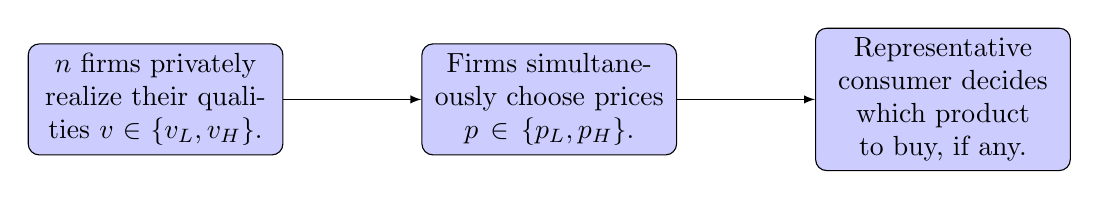
\begin{tikzpicture}[node distance=2cm]
\node (start) [startstop] {$n$ firms privately realize their qualities $v \in \{v_L, v_H\}$.};
\node (pro2b) [startstop, right of=start, xshift=3cm] {Firms simultaneously choose prices $p \in \{p_L, p_H\}$.};
\node (pro2c) [startstop, right of=pro2b, xshift=3cm] {Representative consumer decides which product to buy, if any.};
\draw [arrow] (start) -- (pro2b);
\draw [arrow] (pro2b) -- (pro2c);
\end{tikzpicture}
\caption{Timing of the Game}
\label{timing}
\end{figure}
